\chapter{Valparaiso}
\section*{14 mars 2015}
Après Santiago, nouvelle étape «ville» avec Valparaiso et juste à côté Viña del Mar. \newline
 Valparaiso \newline
 La ville est dans la brume tous les matins. \newline
 \newline
\centerline{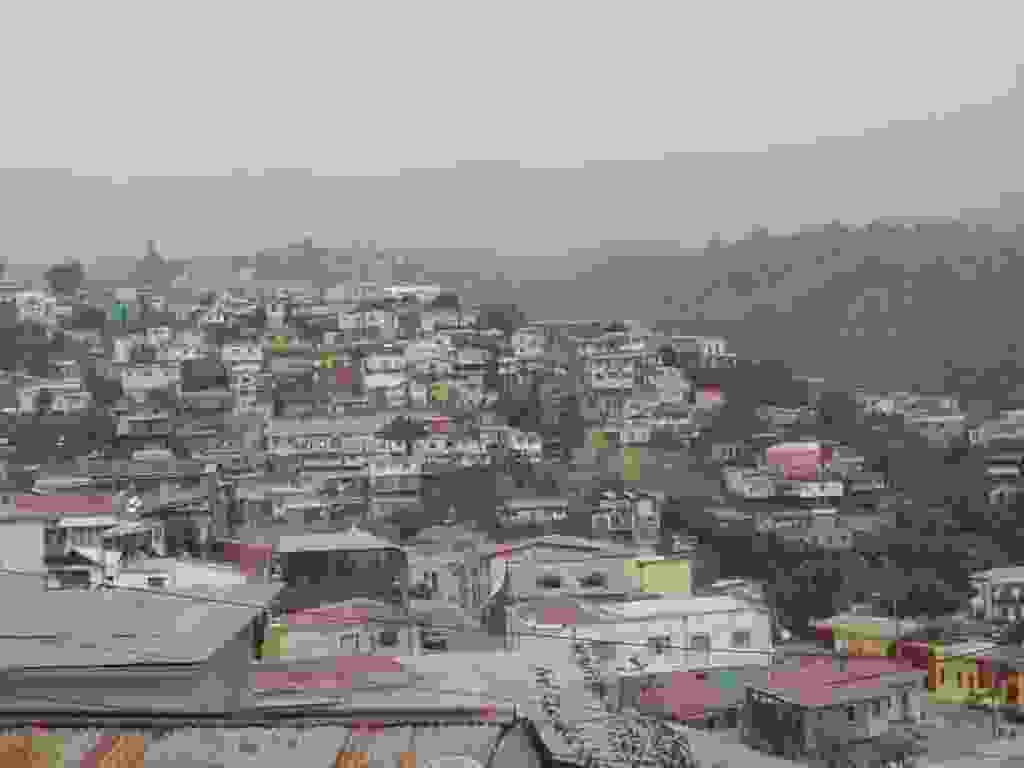
\includegraphics[width=\mywidth]{../wp-content/uploads/2015/03/P3092690-1024x768.jpg} } 
\newline
\centerline{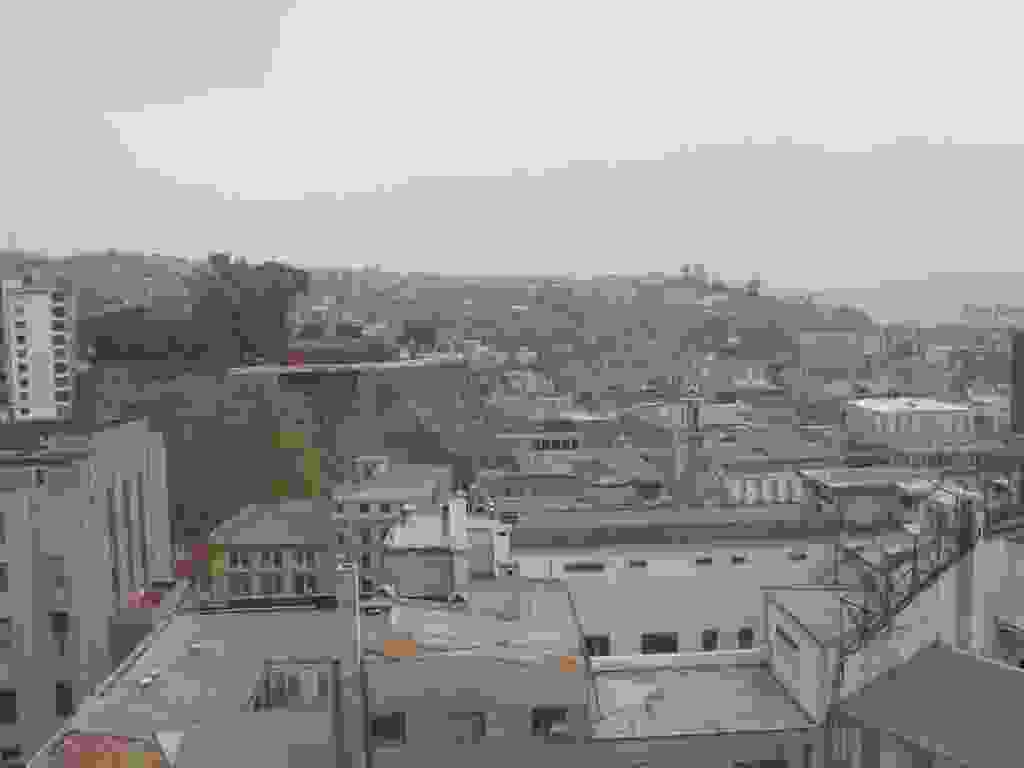
\includegraphics[width=\mywidth]{../wp-content/uploads/2015/03/P30926731-1024x768.jpg} } 
Puis l´après midi ca se dégage. \newline
 \newline
\centerline{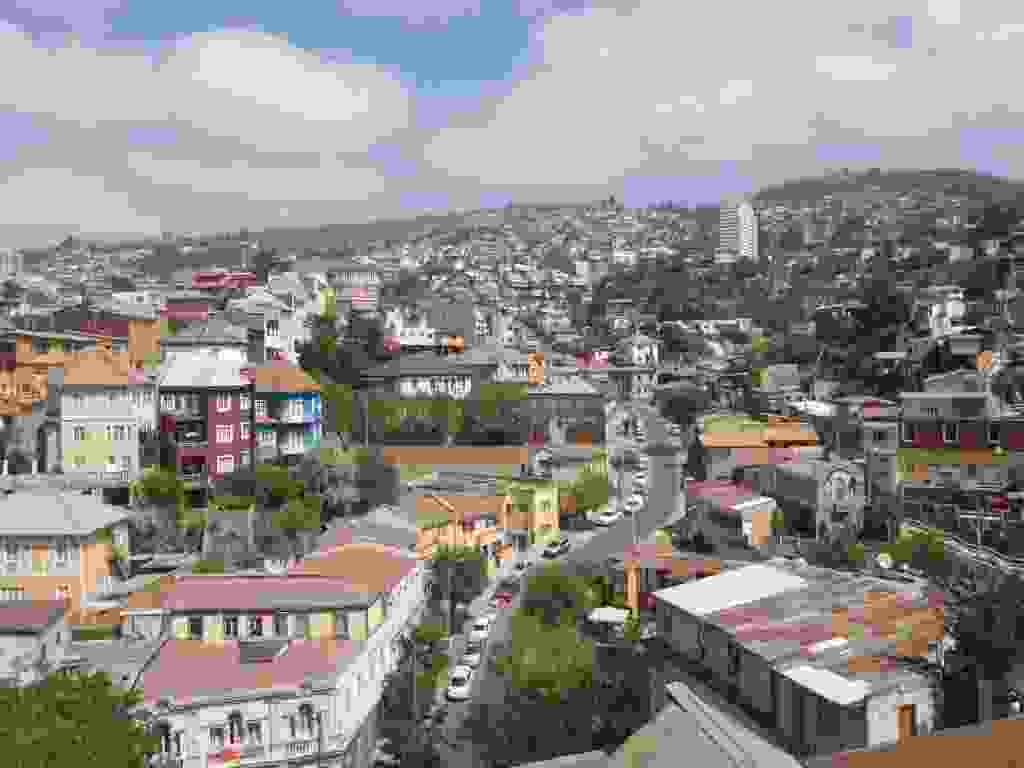
\includegraphics[width=\mywidth]{../wp-content/uploads/2015/03/P3112753-1024x768.jpg} } 
 \newline
\centerline{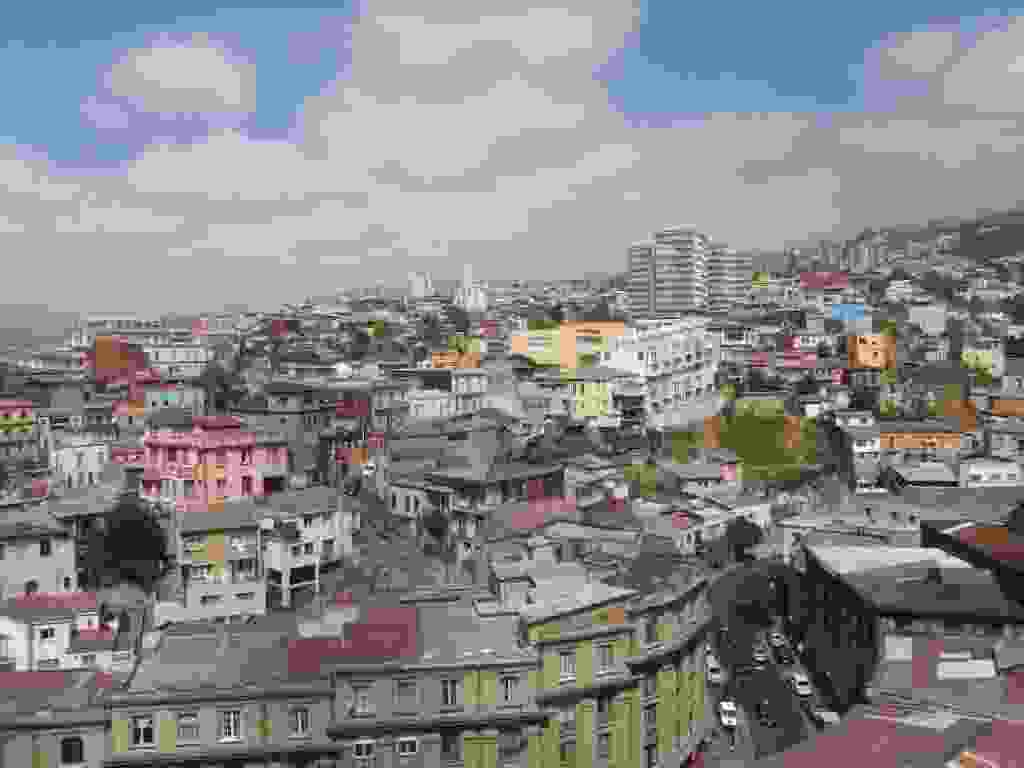
\includegraphics[width=\mywidth]{../wp-content/uploads/2015/03/P3112755-1024x768.jpg} } 
 \newline
\centerline{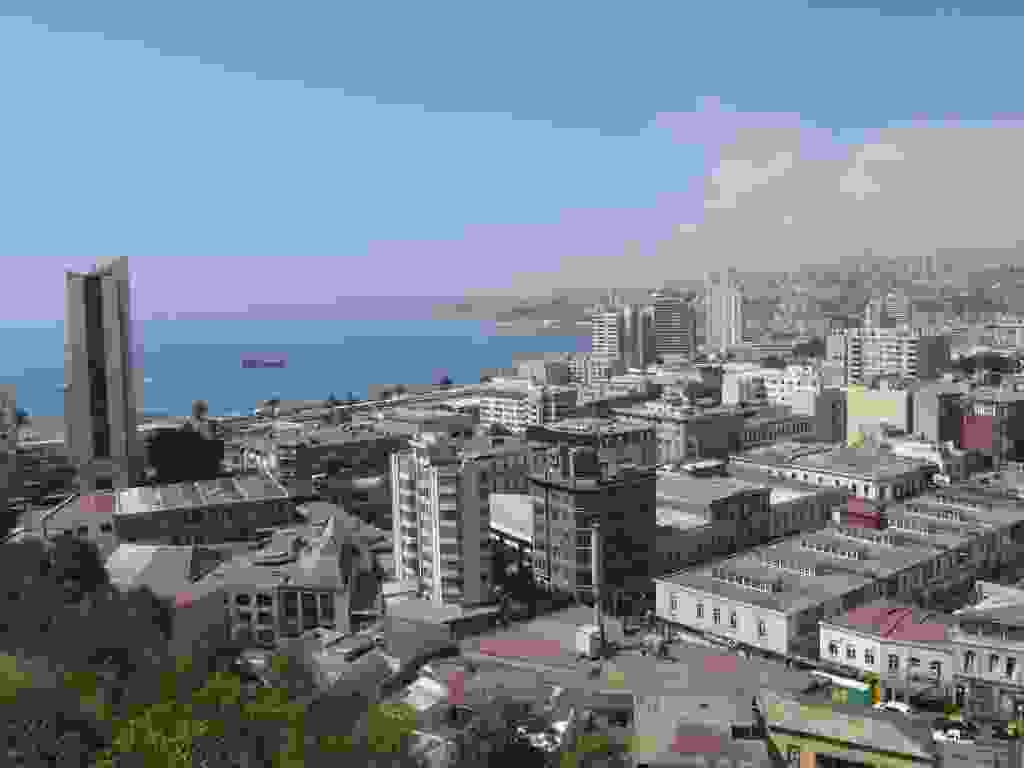
\includegraphics[width=\mywidth]{../wp-content/uploads/2015/03/P3112756-1024x768.jpg} } 
\newline
\centerline{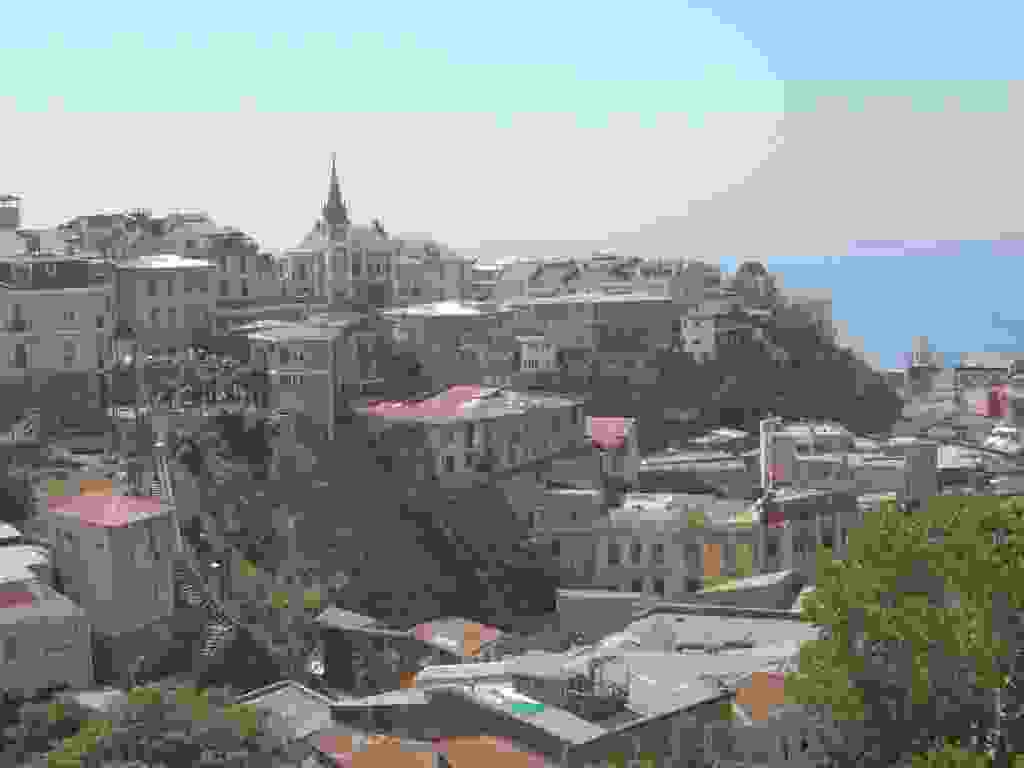
\includegraphics[width=\mywidth]{../wp-content/uploads/2015/03/P3112748-1024x768.jpg} } 
 \newline
\centerline{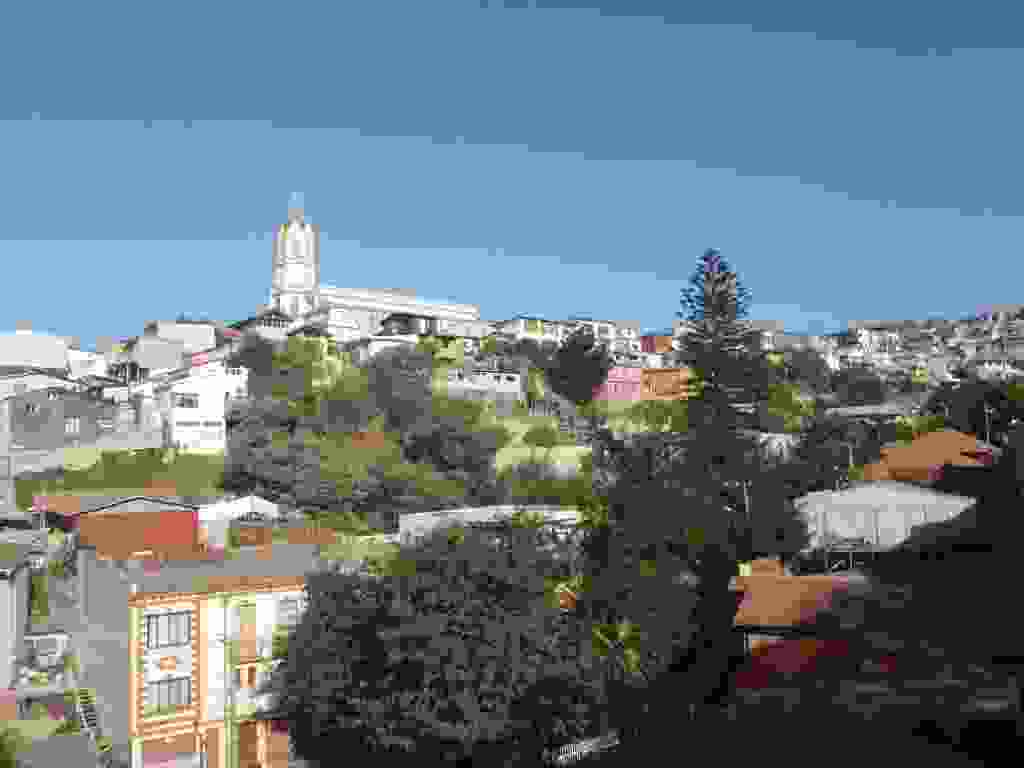
\includegraphics[width=\mywidth]{../wp-content/uploads/2015/03/P3092710-1024x768.jpg} } 
 \newline
\centerline{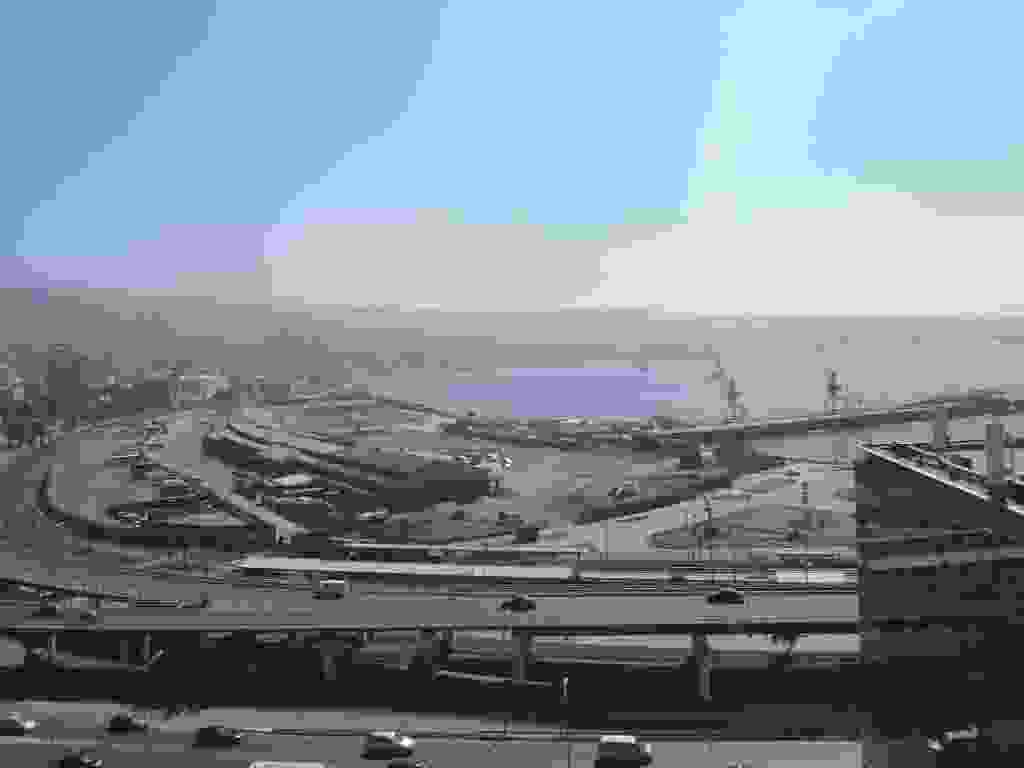
\includegraphics[width=\mywidth]{../wp-content/uploads/2015/03/P3092695-1024x768.jpg} } 
Laville est très colorée avec de nombreuses fresques sur les murs. Il y a aussi des coins assez sales. \newline
 \newline
\centerline{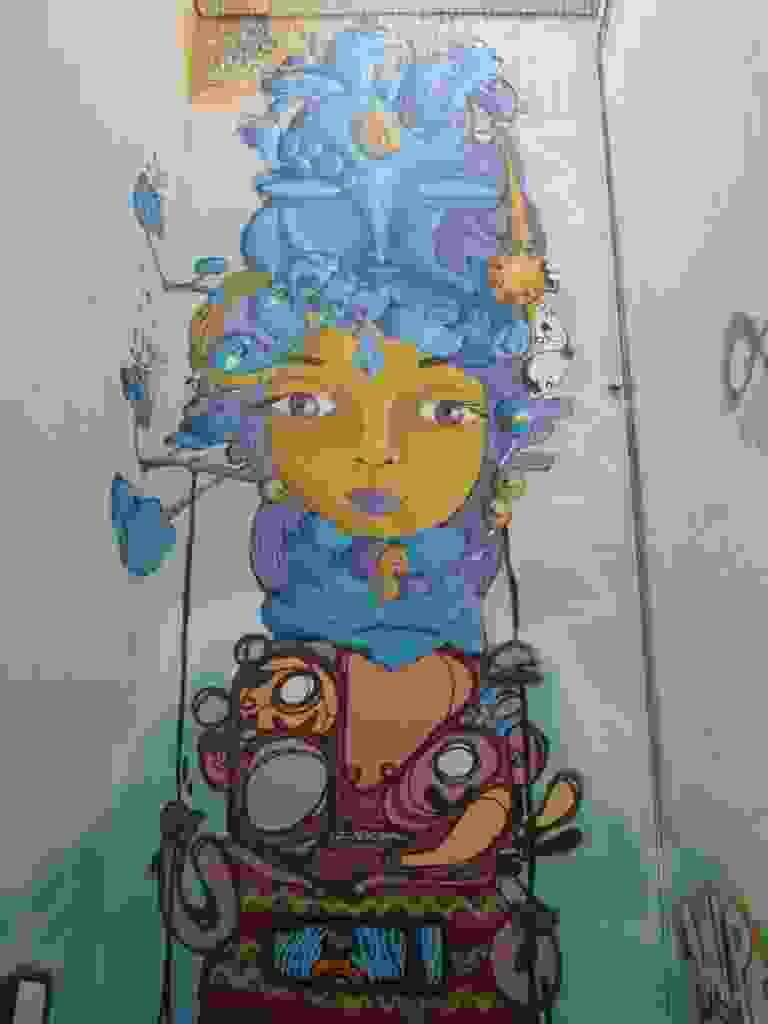
\includegraphics[width=\mywidth]{../wp-content/uploads/2015/03/P3092677-768x1024.jpg} } 
 \newline
\centerline{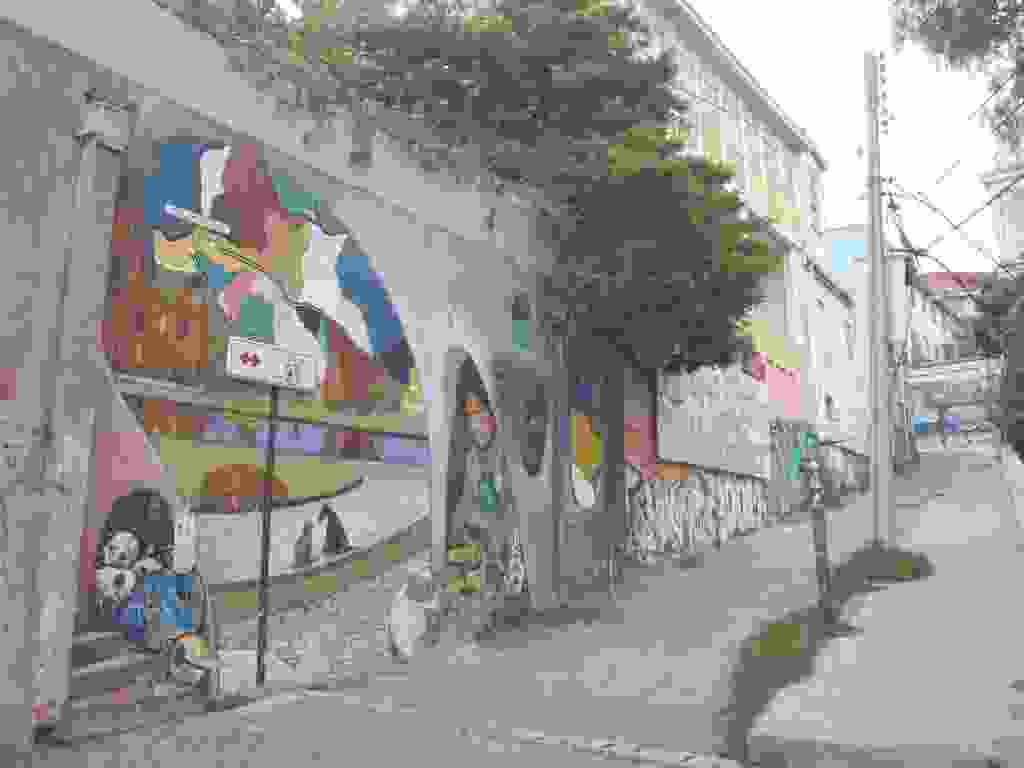
\includegraphics[width=\mywidth]{../wp-content/uploads/2015/03/P3092675-1024x768.jpg} } 
 \newline
\centerline{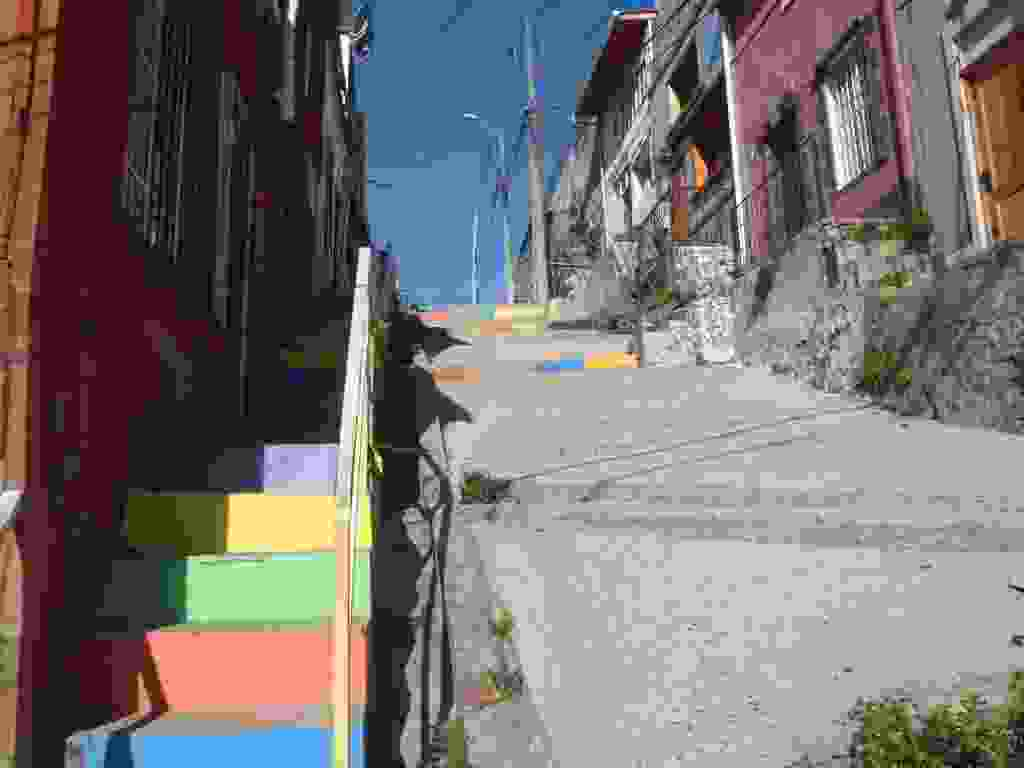
\includegraphics[width=\mywidth]{../wp-content/uploads/2015/03/P3092708-1024x768.jpg} } 
 \newline
\centerline{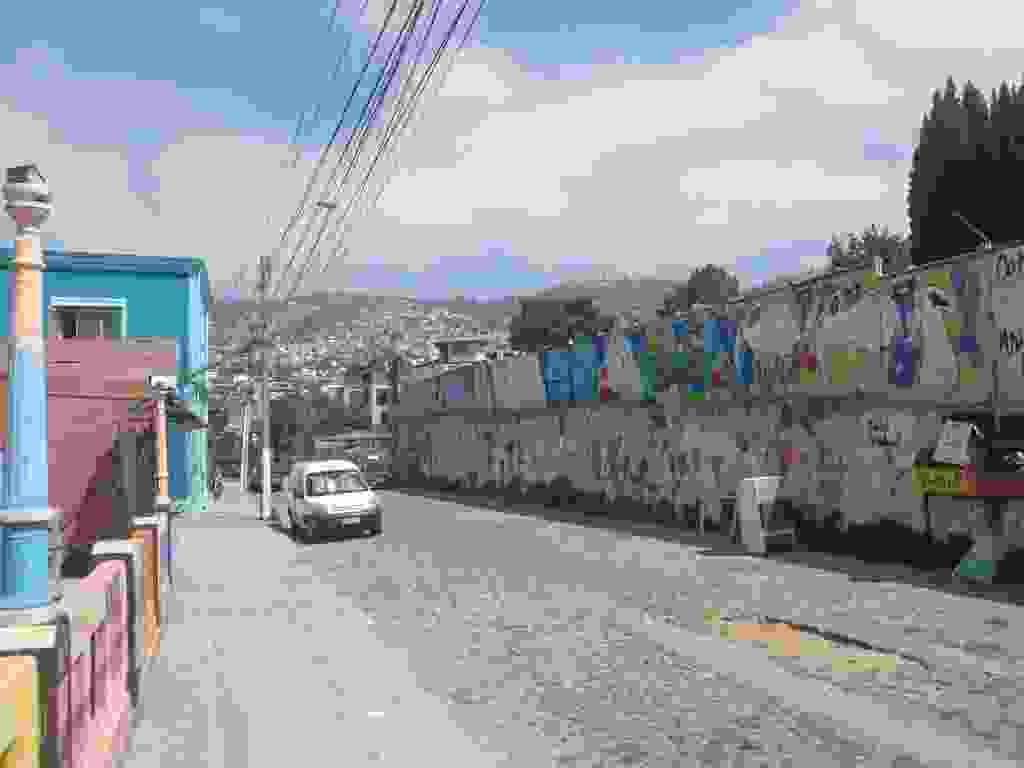
\includegraphics[width=\mywidth]{../wp-content/uploads/2015/03/P3112757-1024x768.jpg} } 
 \newline
\centerline{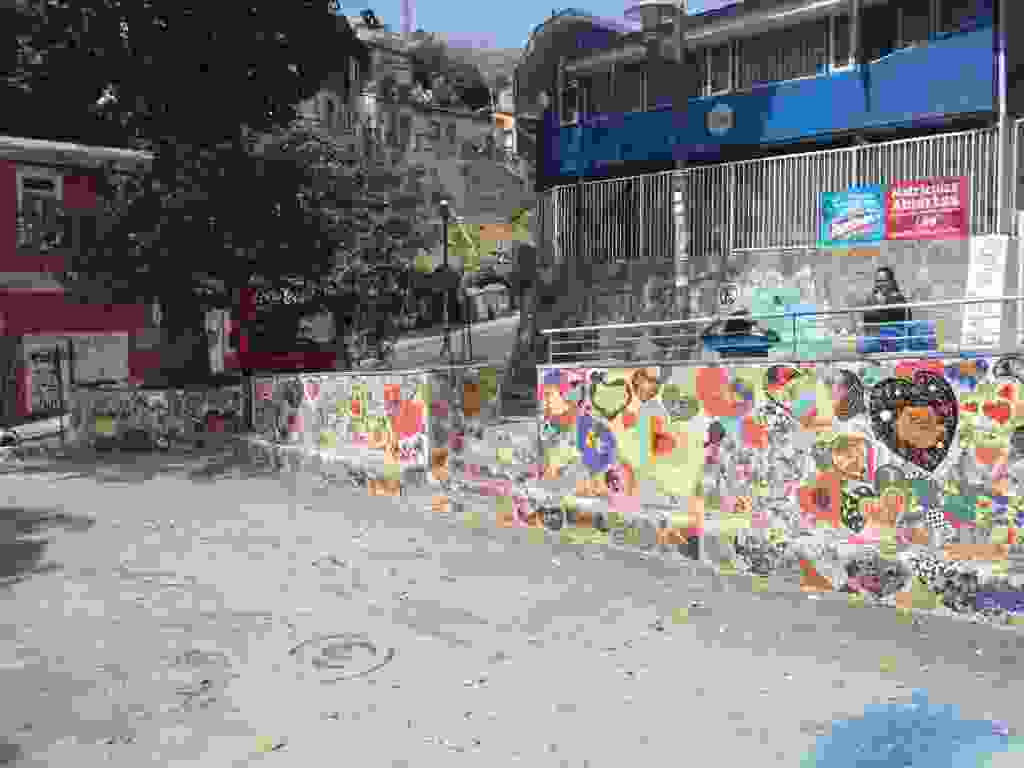
\includegraphics[width=\mywidth]{../wp-content/uploads/2015/03/P3112744-1024x768.jpg} } 
 \newline
\centerline{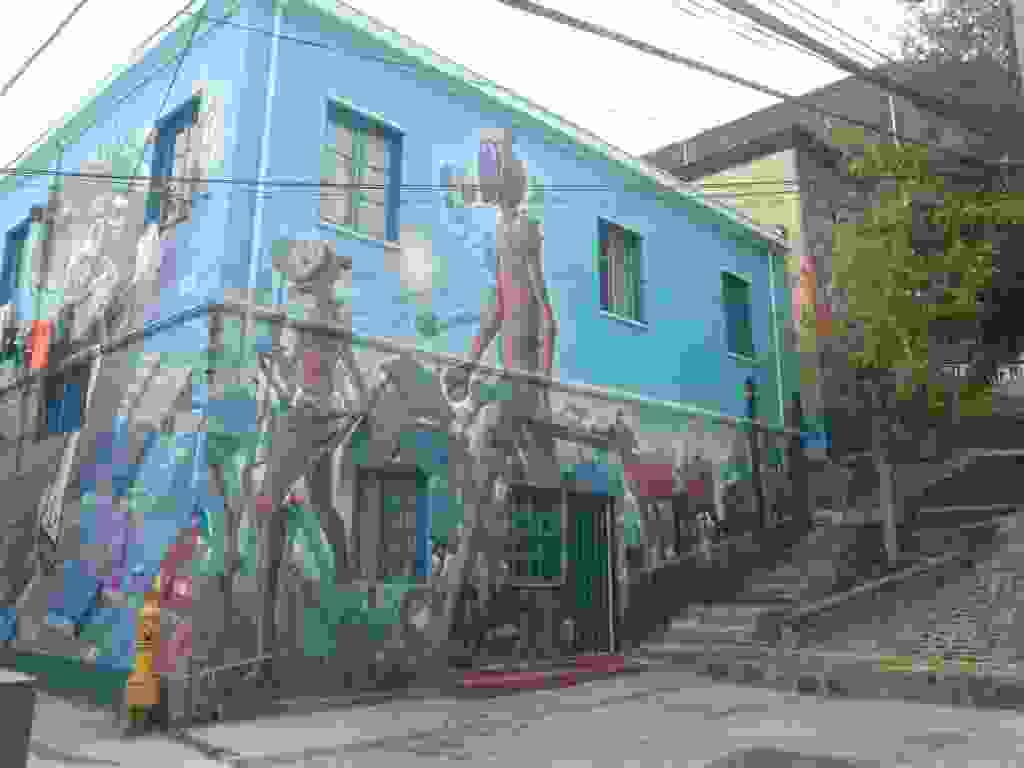
\includegraphics[width=\mywidth]{../wp-content/uploads/2015/03/P3092686-1024x768.jpg} } 
 \newline
 La Plaza Sotomayor en plein centre. \newline
 \newline
\centerline{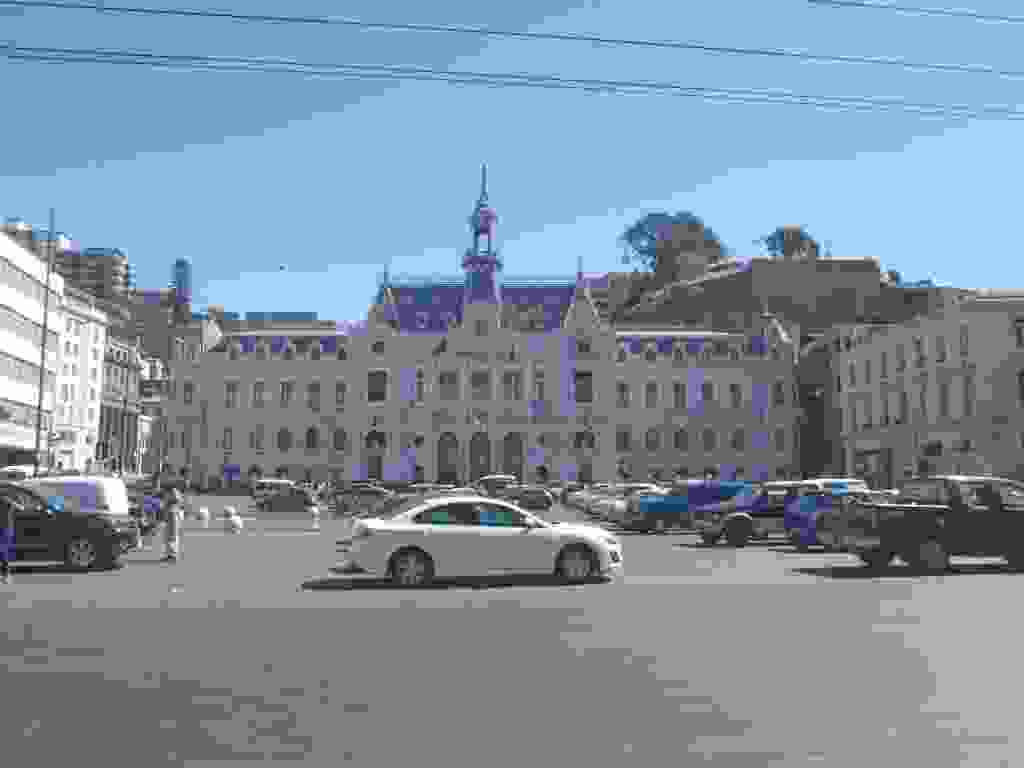
\includegraphics[width=\mywidth]{../wp-content/uploads/2015/03/P3082665-1024x768.jpg} } 
 \newline
\centerline{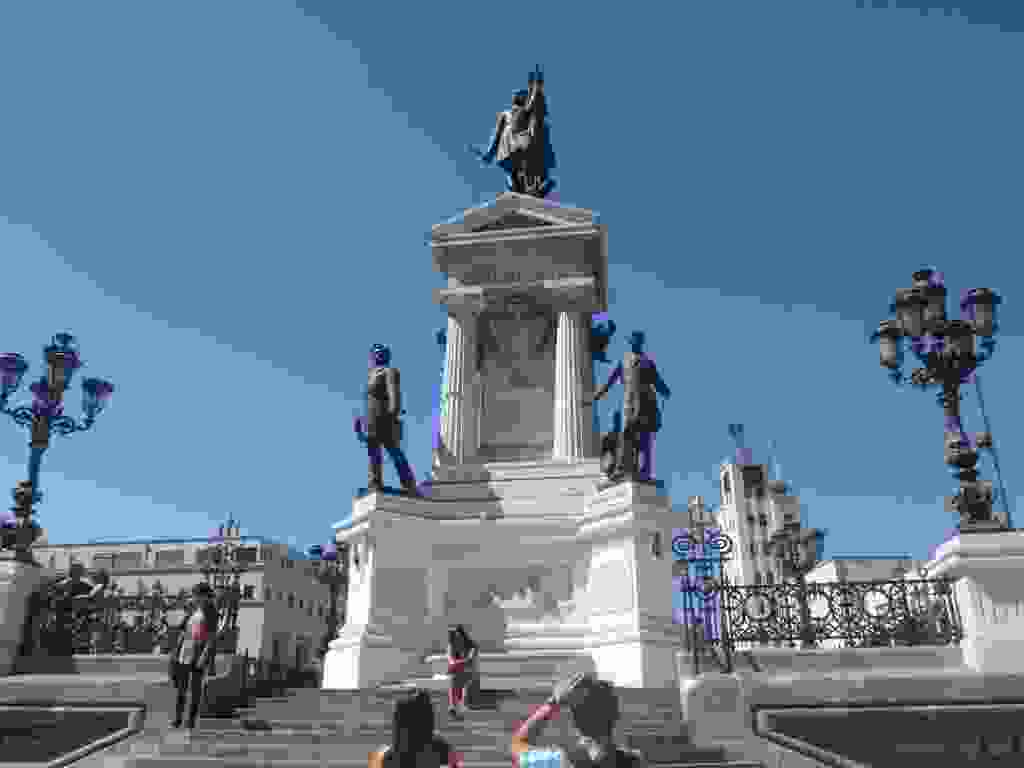
\includegraphics[width=\mywidth]{../wp-content/uploads/2015/03/P3082666-1024x768.jpg} } 
 \newline
 De multiples petits funiculaires permettent d'accéder aux hauteurs de la ville. \newline
 \newline
\centerline{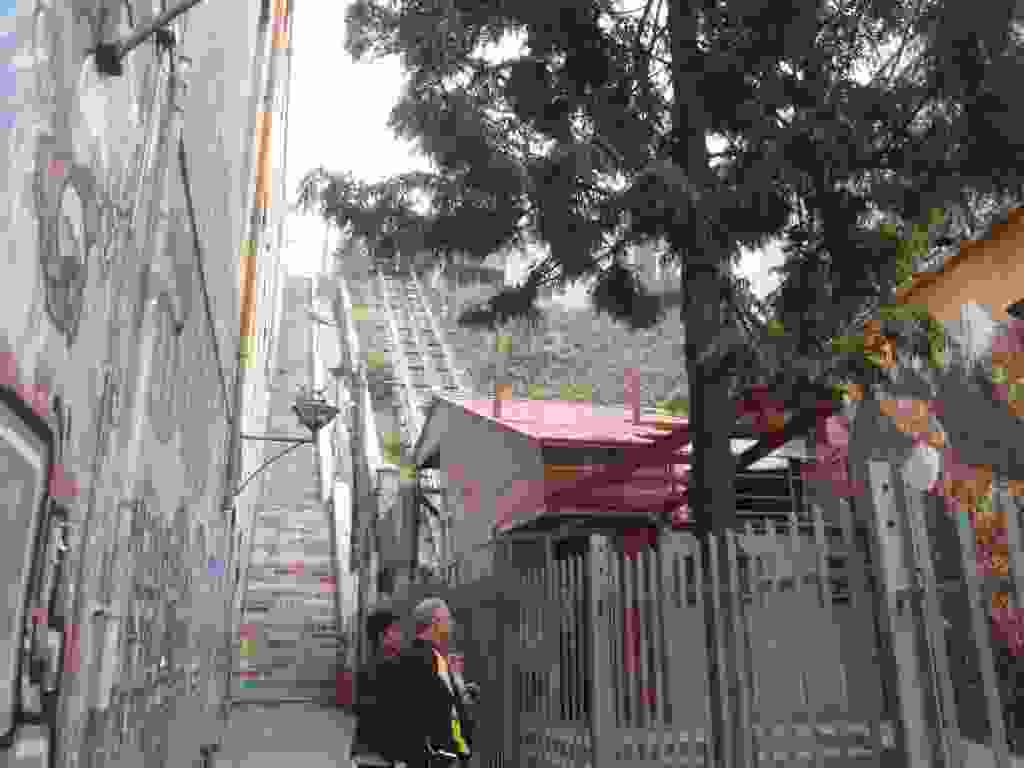
\includegraphics[width=\mywidth]{../wp-content/uploads/2015/03/P3092679-1024x768.jpg} } 
 \newline
\centerline{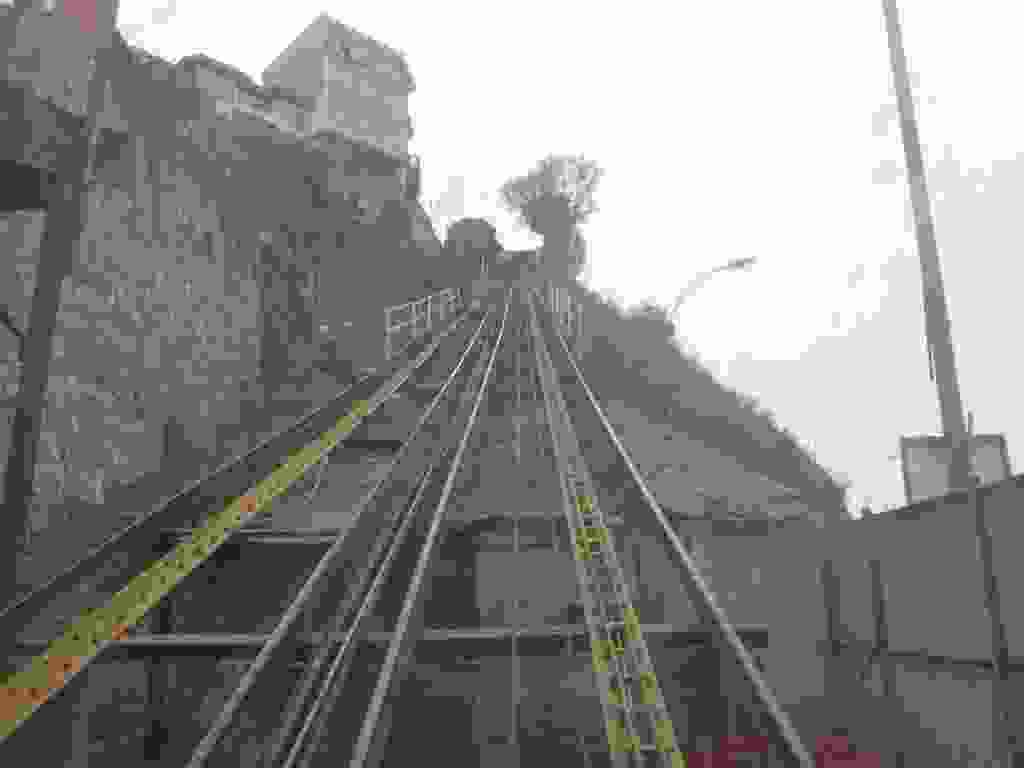
\includegraphics[width=\mywidth]{../wp-content/uploads/2015/03/P3092682-1024x768.jpg} } 
 \newline
\centerline{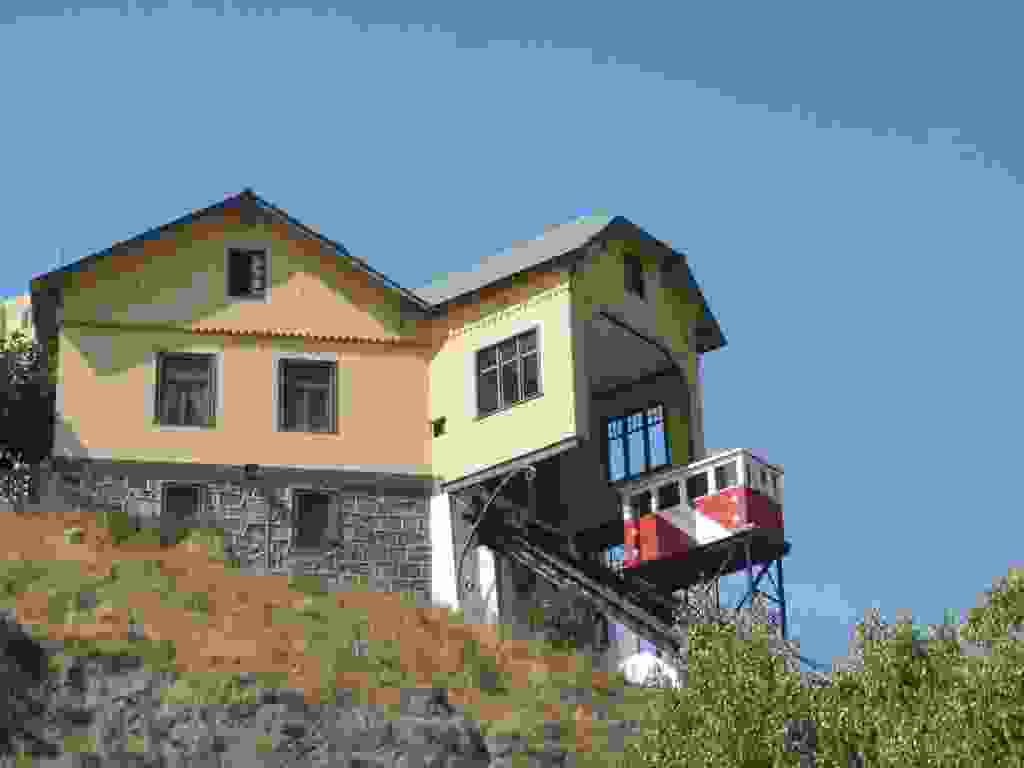
\includegraphics[width=\mywidth]{../wp-content/uploads/2015/03/P3092693-1024x768.jpg} } 
Le marché aux fruits. \newline
 \newline
\centerline{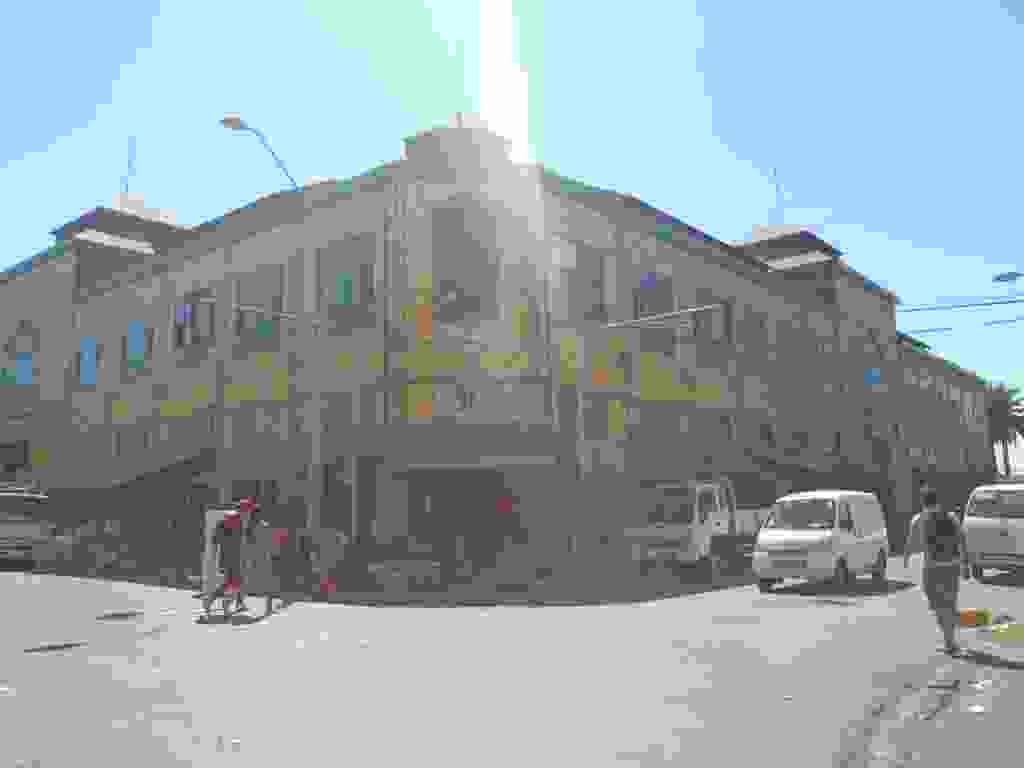
\includegraphics[width=\mywidth]{../wp-content/uploads/2015/03/P3082664-1024x768.jpg} } 
Ils font du bon boulot !\newline
\centerline{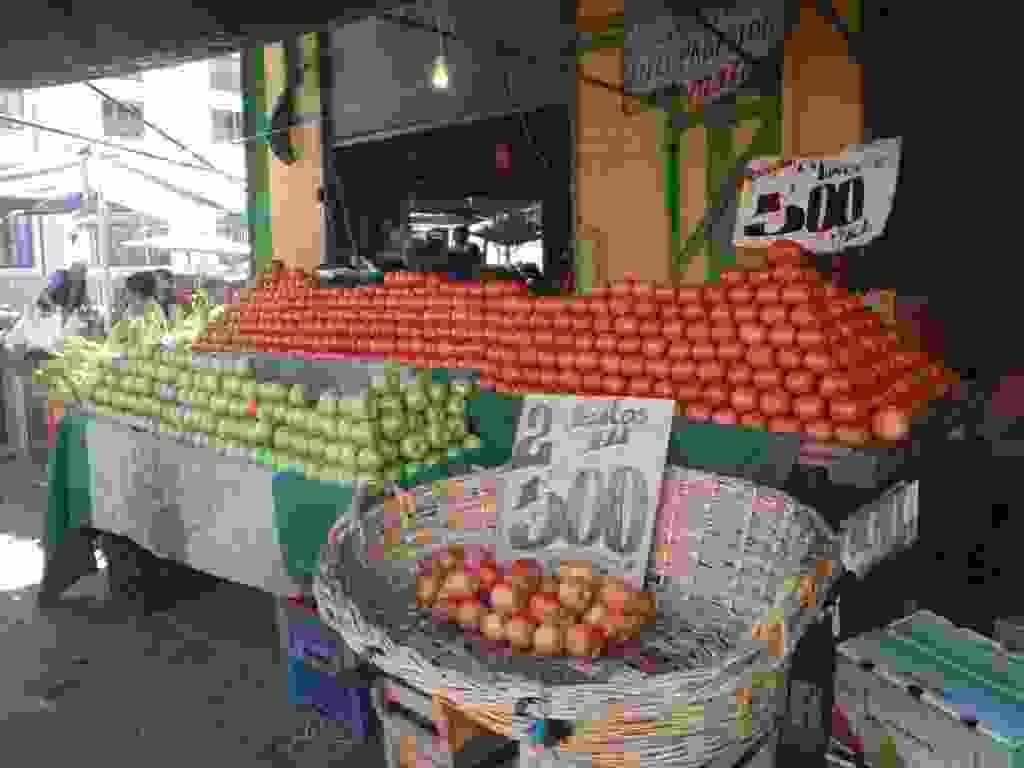
\includegraphics[width=\mywidth]{../wp-content/uploads/2015/03/P3092698-1024x768.jpg} } 
 \newline
 L´hostel oú j´ai logé à Valparaiso, tenu par un francais et aussi avec beaucoup de client francais. \newline
 \newline
\centerline{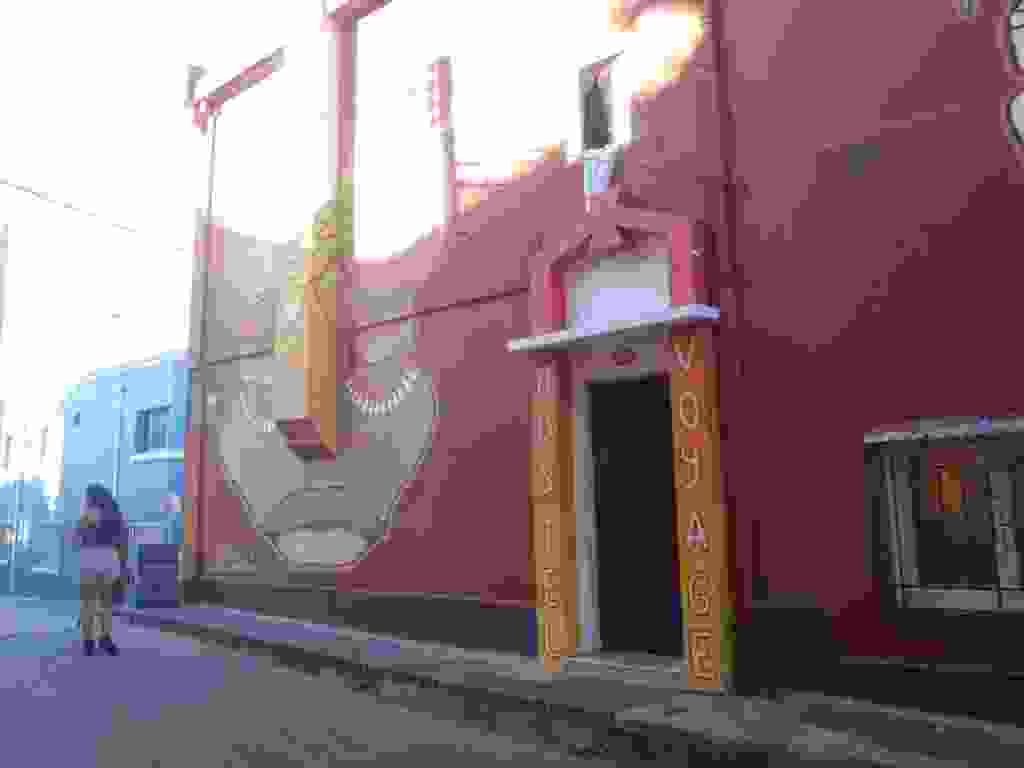
\includegraphics[width=\mywidth]{../wp-content/uploads/2015/03/P3092668-1024x768.jpg} } 
 \newline
 Un soir, un chilien a préparé un superbe plat de fruits de mer, poulet et pommes de terre. Le tout cuit au feu de bois, un régal ! \newline
 \newline
\centerline{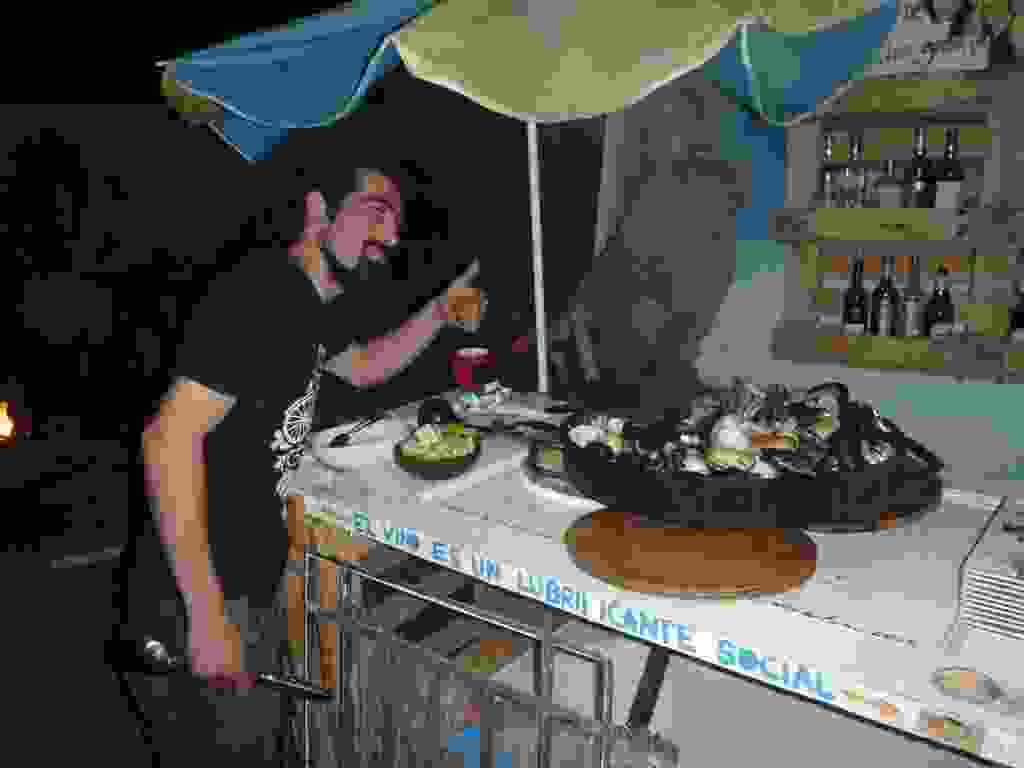
\includegraphics[width=\mywidth]{../wp-content/uploads/2015/03/P3112743-1024x768.jpg} } 
 \newline
 \newline
\centerline{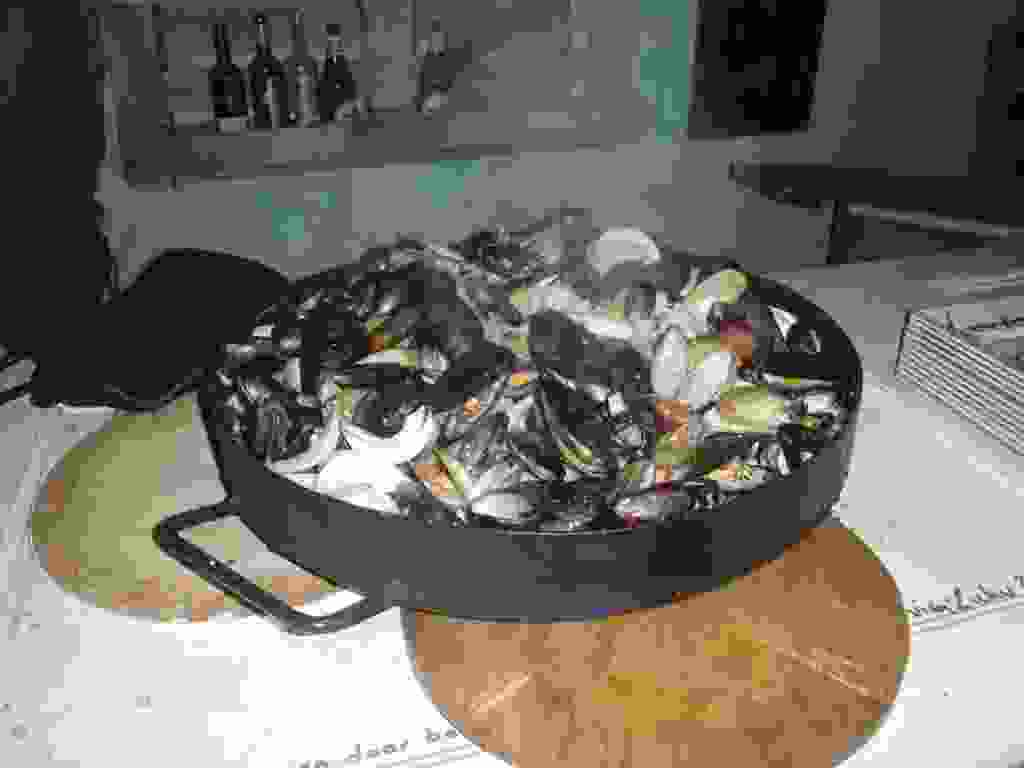
\includegraphics[width=\mywidth]{../wp-content/uploads/2015/03/P3112742-1024x768.jpg} } 
 \newline
 Viña del Mar \newline
 A peine à 10km de Valparaiso mais avec une ambiance totalement différente, ville balnéaire très propre avec de belles plages et des grands immeubles face à la mer. \newline
 \newline
\centerline{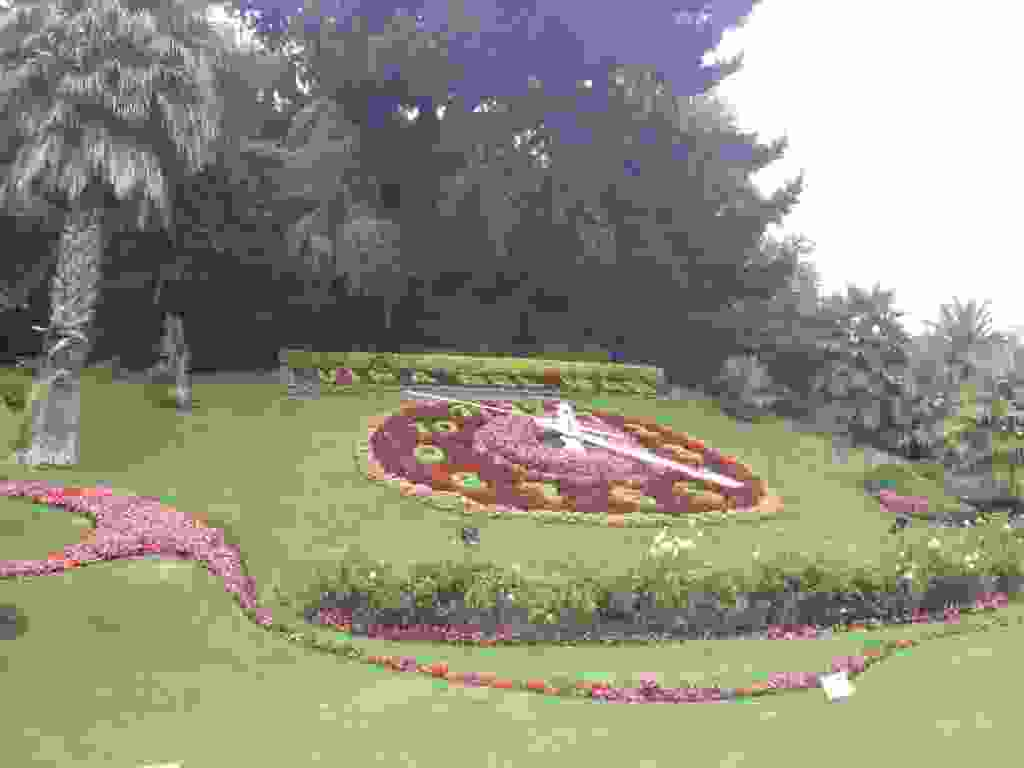
\includegraphics[width=\mywidth]{../wp-content/uploads/2015/03/P3102721-1024x768.jpg} } 
 \newline
\centerline{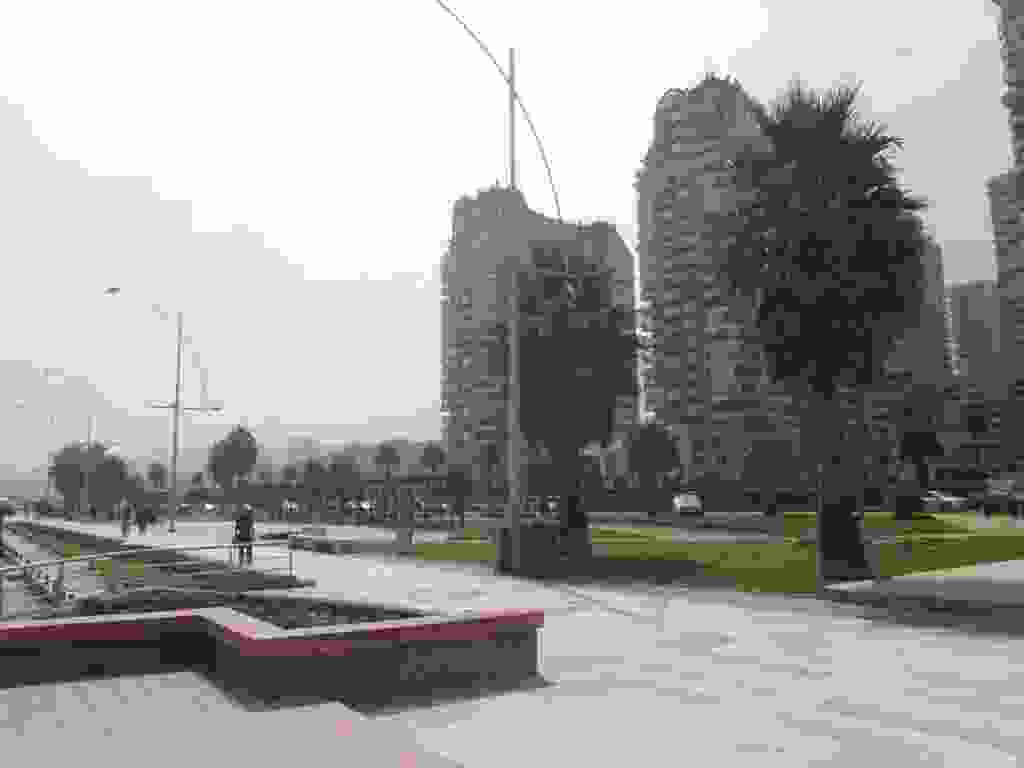
\includegraphics[width=\mywidth]{../wp-content/uploads/2015/03/P3102726-1024x768.jpg} } 
 \newline
\centerline{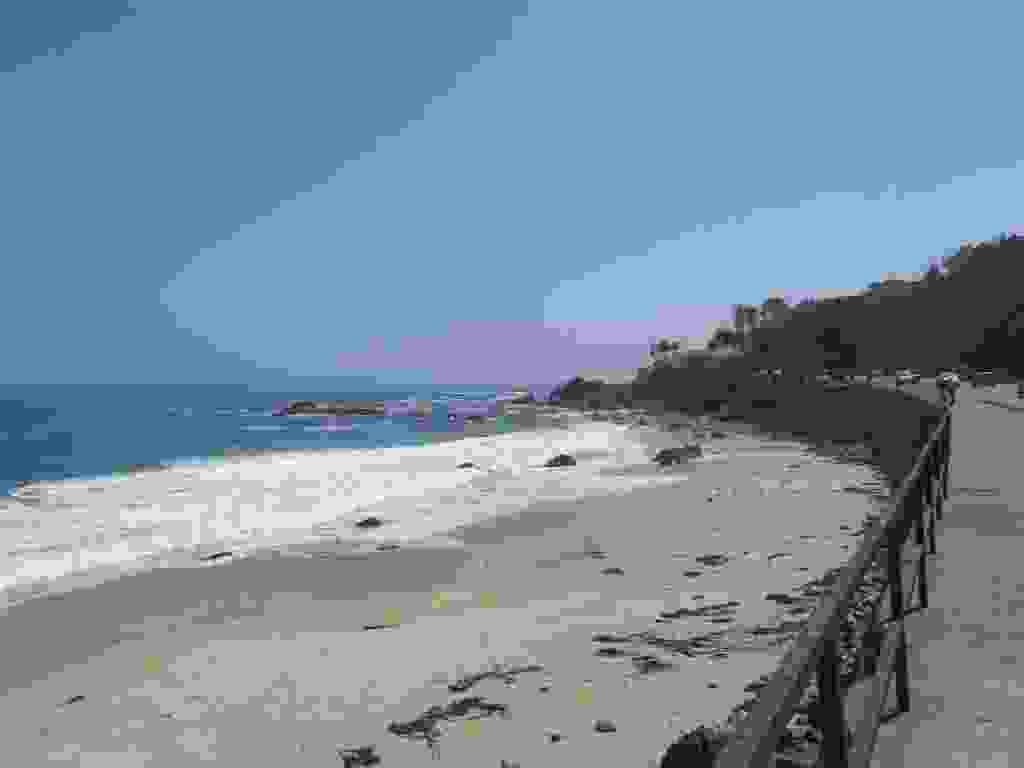
\includegraphics[width=\mywidth]{../wp-content/uploads/2015/03/P3102728-1024x768.jpg} } 
 \newline
\centerline{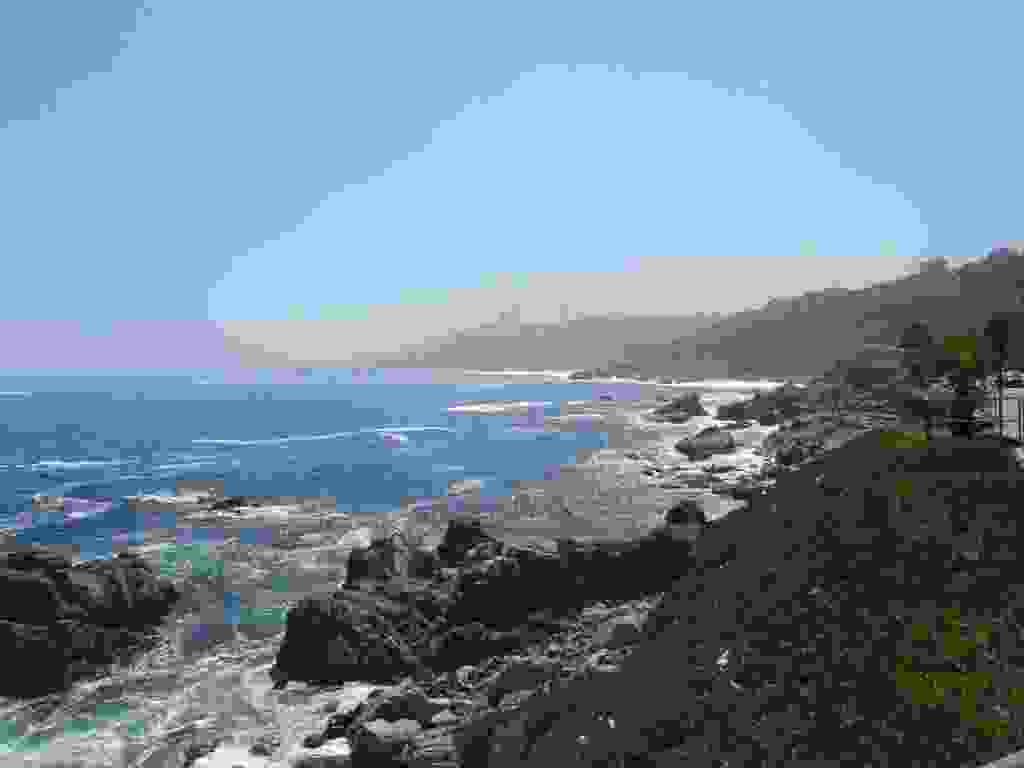
\includegraphics[width=\mywidth]{../wp-content/uploads/2015/03/P31027291-1024x768.jpg} } 
 \newline
\centerline{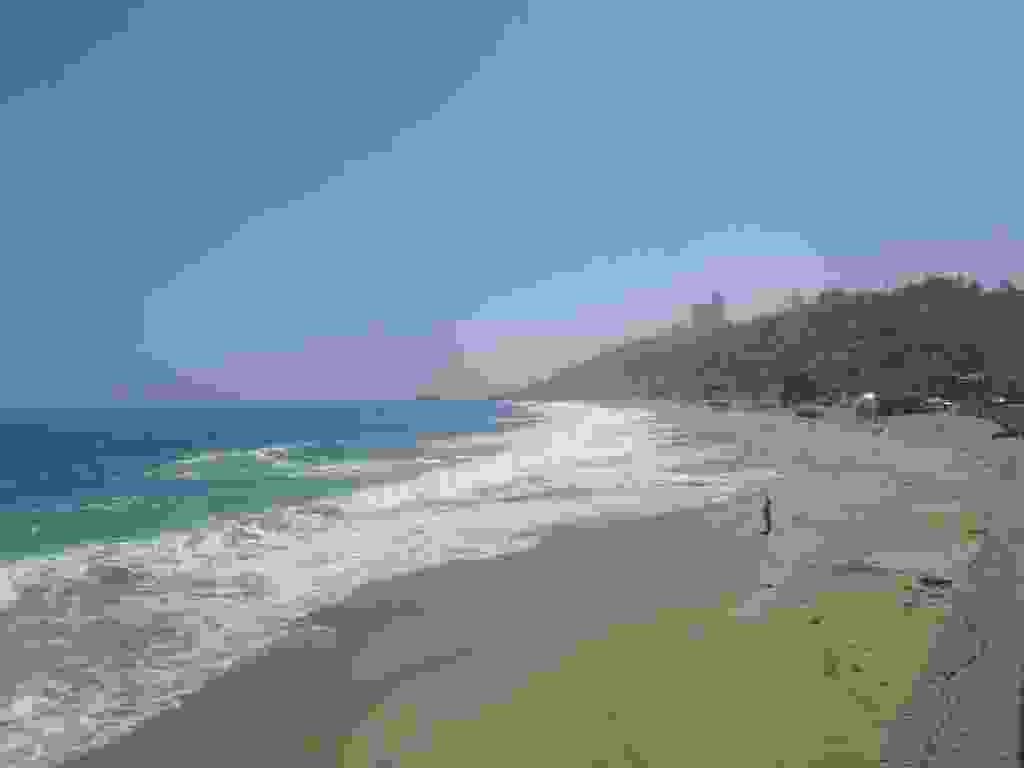
\includegraphics[width=\mywidth]{../wp-content/uploads/2015/03/P3102731-1024x768.jpg} } 
 \newline
\centerline{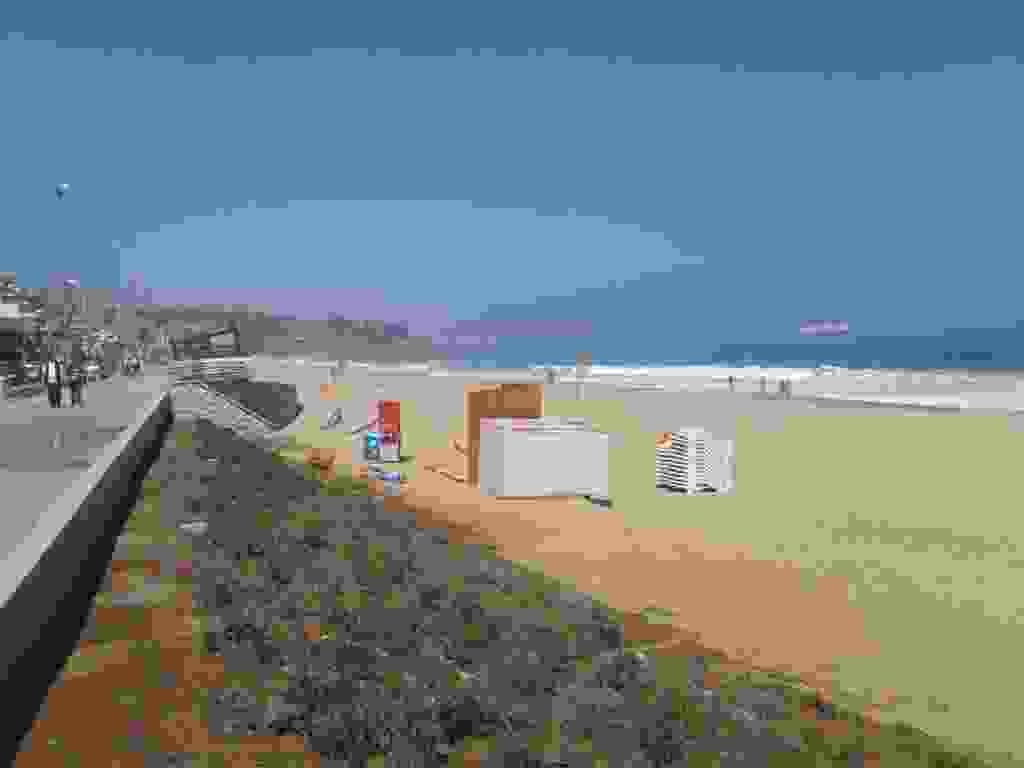
\includegraphics[width=\mywidth]{../wp-content/uploads/2015/03/P3102732-1024x768.jpg} } 
 \newline
\centerline{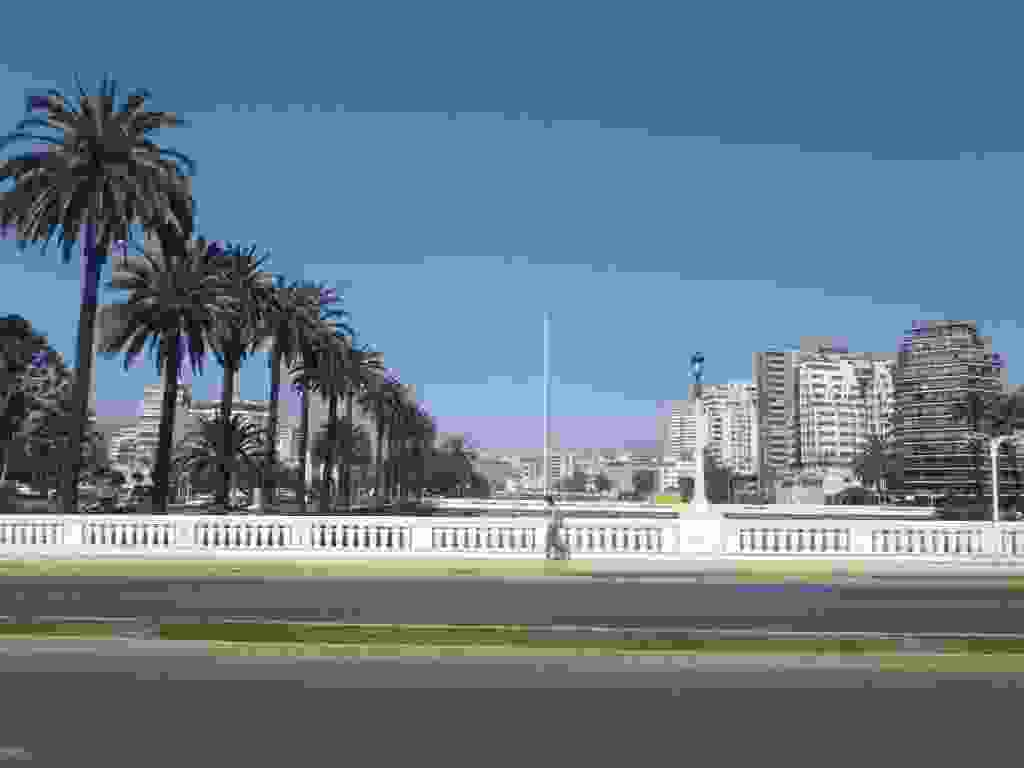
\includegraphics[width=\mywidth]{../wp-content/uploads/2015/03/P3102735-1024x768.jpg} } 
 \newline
\centerline{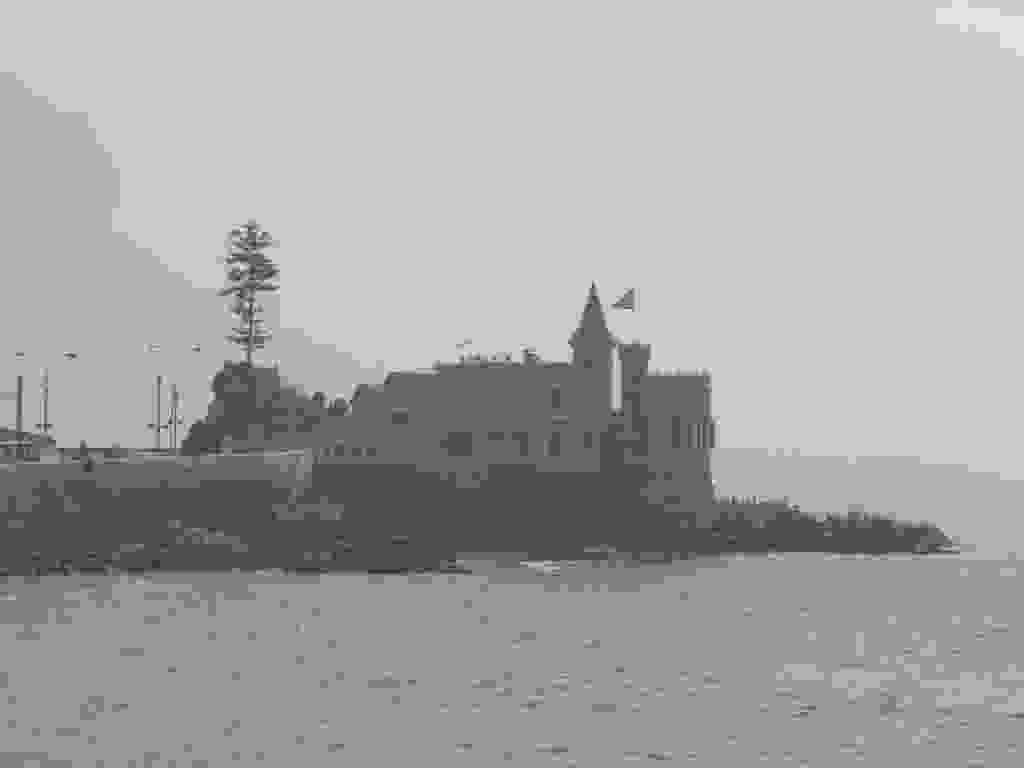
\includegraphics[width=\mywidth]{../wp-content/uploads/2015/03/P3102738-1024x768.jpg} } 
 \newline
\centerline{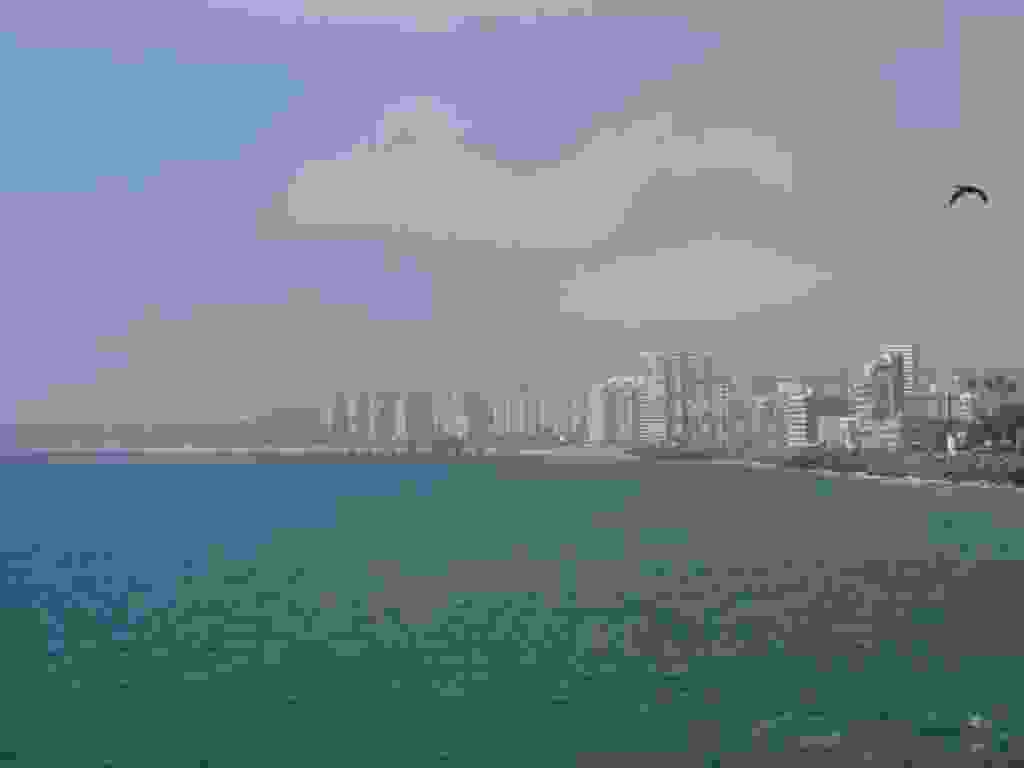
\includegraphics[width=\mywidth]{../wp-content/uploads/2015/03/P3102739-1024x768.jpg} } 
 \newline
\centerline{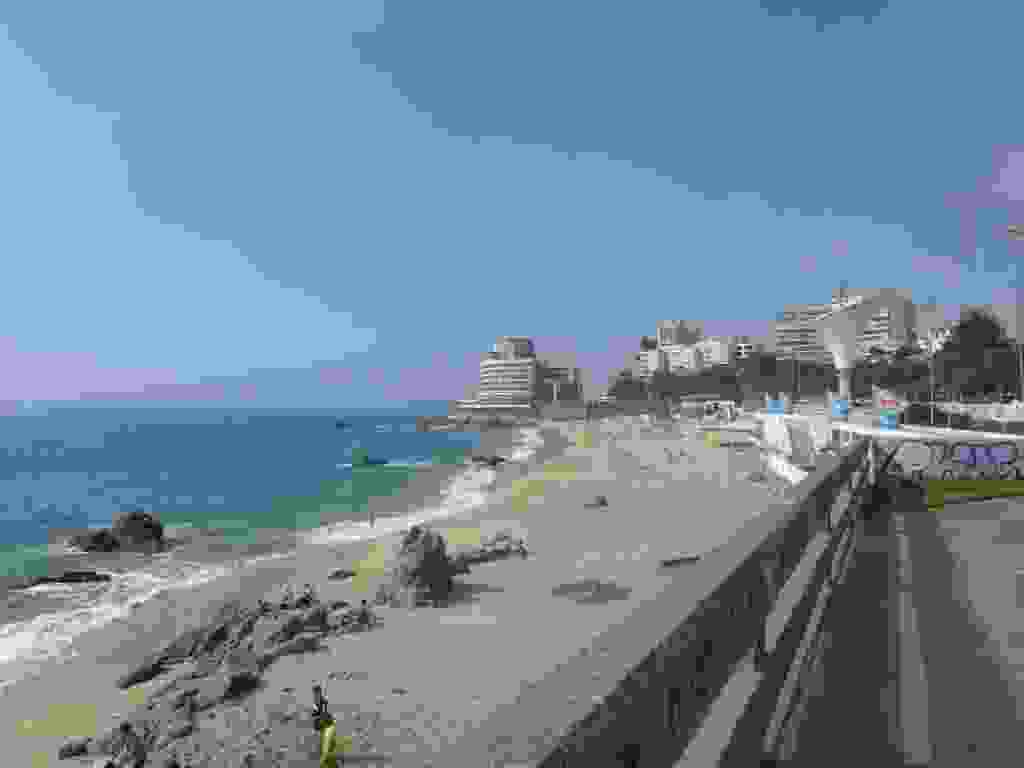
\includegraphics[width=\mywidth]{../wp-content/uploads/2015/03/P3102741-1024x768.jpg} } 
 \newline

\newpage
 
